
\section{Neutrons in Super-Kamiokande}
\label{sec:sk_neutron}

Super-Kamiokande and other large scale water Cherenkov detectors have provided %
much evidence in the experimental understanding of neutrinos, %
be it originated in solar, atmospheric, or accelerator facilities.
Despite the large exposure of the experiment, some studies are still curbed by statistical uncertainty %
and would benefit from simply collecting more data.
Other searches, instead, suffer from irreducible background events, as for example the detection of Supernova Relic Neutrinos (SRN), %
%One of the main motivation to detect neutrons is to be able to detect relic supernova neutrinos, %
an incoherent background spectrum produced from all previous core-collapse supernova explosions in the Universe (see \refsec{sec:nu_sun_sn}).
The observation of SRN would be of great importance for improving our knowledge on the population of core-collapse SN %
and the rate of star formation.
The average energies of these neutrinos are around a few tens of MeV, at which the largest cross-section %
corresponds to inverse beta decay (IBD, see \reffig{sec:xsec}).
%which is two orders of magnitude larger than $\nu_e$ elastic scattering.
This measurement is afflicted for energies between $14\,\text{MeV} < E_\nu < 30\,\text{MeV}$ %
by nonrelativistic muons produced from atmospheric neutrinos which are below Cherenkov threshold and decay into electrons, %
known as \emph{invisible muon decays}~\cite{Kaplinghat:1999xi}.
At lower energy, the dominant backgrounds are decays of muon-induced spallation products, %
between 10\,MeV and 18\,MeV, and reactor neutrinos below 10\,MeV.
No SRN has been detected yet~\cite{Bays:2011si, Zhang:2013tua}, but %
theoretical predictions place the diffuse supernova neutrino background flux (DSNB, see \refsec{sec:nu_sun_sn}) %
within a factor of four below the upper limit obtained by SK in 2003~\cite{Malek:2002ns, Horiuchi:2008jz}.
Even though a more recent and detailed analysis with increased efficiency, lower energy threshold, and expanded statistics %
revealed less stringet limits~\cite{Bays:2011si}, neutron tagging capabilities could reduce %
the invisible muon background by a factor of five and remove the spallation background.
%upper limits on supernova relic neutrino flux are between 2.8 and 3:1 e cm2 s1 > 16 MeV total
%positron energy (17.3 MeV E).


Searches of galactic supernova bursts could also avail of an improved background suppression.
SK will be exposed to a huge number of neutrino events if a core-collapse supernova occurs inside our galaxy.
Such an event would provide not only an early warning system for other observatories, %
but also information about the neutrino spectrum, time profile, and information about early stages of the core-collapse process, %
like pre-supernova neutrinos from the silicon burning phase~\cite{Simpson:2019xwo}.
A sizeable amount of the neutrinos emitted are actually antineutrinos in the energies where the IBD cross-section dominates.
%(see \reffig{fig:xsec}).
Detecting the neutron in the final state is fundamental for distinguishing whether the incoming particle is %
a neutrino or an antineutrino.
Improved neutron tagging is also helpful to understand atmospheric and accelerator neutrino interactions and final states.
At energies $E_\nu > 1$\,GeV, the number of CCQE interactions decreases and often additional neutrons %
from $2p2h$ interactions or pions from baryon resonance are also released in the scattering process.
The possibility of separating neutrinos and antineutrinos can nevertheless improve the purity of antineutrino samples.
Finally, neutron-induced background in proton decay searches can be reduced, %
since most channels do not require neutrons to appear in the final state.
%since it requires no neutrons to appear in the final state.

%Among these background sources, flasher events\footnote{A flasher event refers to the phenomenon %
%	in which a PMT mis-fires and many repetitive internal discharges are triggered also on nearby PMTs.
%	Flasher events tend to have a broader hit timing distribution than neutrino events.} %

\subsection{Neutron tagging}

Neutrons have a relative long lifetime and, since they cannot directly emit Cherenkov radiation, %
these particles can travel quite some distance from their production point without being detected.
Neutrons interact with nuclei in various ways, depending on their energy and the target nucleus.
The interactions are divided in three typologies: scatterings, which can be elastic or inelastic, %
absorptions, such as radiative capture or fission, and nucleon transfer reactions.
The kinetic energy of the neutron $T$, sometimes referred to as the \emph{detection temperature}, %
is the main factor in determining the dominant cross-section of these interactions.
For fast neutrons, with $T > 1$\,MeV, elastic scattering is the prevailing interaction mode, and %
for some target nuclei the only mode possible.
The cross-section for these energetic neutrons present some wide resonance peaks which depend %
on the target nuclei.
The elastic scattering cross-section at energies below 1\,MeV is almost independent of the neutron energy.
This is true for most light isotopes, but some intermediate and heavy elements present some specific %
behaviour at higher energy.
Neutrons for which $T \simeq \np{0.025}$\,eV are called \emph{thermal neutrons} because %
a Maxwell-Boltzmann distribution at the temperature of 290\,K peaks at that energy; %
such neutrons are in thermal equilibrium with the surrounding medium.
At thermal energies and below, the most important interaction is neutron absorption, %
the cross-section of which follows the ``$1/v$ law'', with $v$ the velocity of the neutron.
In this region, absorption cross-section increases as the velocity, or the detection temperature, of the neutron decreases
\begin{equation}
	\label{eq:abs_xsec}
	\sigma \sim \frac{1}{v} \sim \frac{1}{T}\ .
\end{equation}
Being in thermal equilibrium and having a lower kinetic energy allows the neutron to form %
a compound nucleus with the target, which might undergo fission or radiation emission if it is a nonfissile nuclide.
For energies between a few eV and hundreds of keV there are resonances in the capture cross-section which %
are strongly dependent on the target isotope, but also on the temperature of the material.
In fact, the thermal motions of the target relative to the incident neutron broadens the resonance peaks, %
despite the integrated cross-section over the energy remains constant.
This effect is called \emph{Doppler broadening}, and results in a decreased likelihood of capture or fission %
when the target material has a wide energy distribution.

%%https://doi.org/10.1016/j.nds.2018.02.001
%BBrown:2018jhjrown:2018jhj,

Fast neutrons slow down to thermal energies via subsequent elastic collisions, until %
the free neutron is captured by some nucleus.
This process is called \emph{thermalisation}.
Considering a scattering between a neutron and a nucleus, $n + A \to n + A$, %
the final state energy of the neutron depends on the outgoing angle $\hat\theta$ %
in the centre of mass frame
\begin{equation}
	\label{eq:outgoing_E}
	E_\text{f} = E_\text{i}\ \frac{(1+\zeta) + (1 - \zeta) \cos\hat\theta}{2} \ ,
\end{equation}
where $E_\text{i,f}$ are the initial and final energies of the free neutron and $\zeta$ %
is the following kinematic factor
\begin{equation}
	\label{eq:n_alpha}
	\zeta = \frac{(m_n - M_A)^2}{(m_n + M_A)^2} \simeq \frac{(1 - A)^2}{(1 + A)^2}\ .
\end{equation}
Using classic mechanics, the scattering angle $\theta$ in the laboratory frame is given by
\begin{equation}
	\label{eq:lab_angle}
	\cos\theta = \frac{A\,\cos\hat\theta + 1}{\sqrt{1 + 2\,A\,\cos\hat\theta + A^2}}\ ,
\end{equation}
and the average scattering angle can be therefore estimated as
\begin{equation}
	\label{eq:average_angle}
	\expval{\cos\theta} = \frac{\displaystyle \int\dd{\Omega} \cos\theta}{\displaystyle \int \dd{\Omega}} = \frac{2}{3 A}\ .
\end{equation}
Heavy targets will deviate on average more the neutron from its path than light targets.
For hydrogen ($A = 1$), the average angle is $\expval{\theta} \simeq 48^\circ$, but %
for heavier elements with large atomic mass, the average angle approximate $\expval{\theta} \to 90^\circ$.
Assuming uniform isotropic scattering, the average outgoing energy for the neutron is
\begin{equation}
	\label{eq:average_outgoing_E}
	\expval{E_\text{f}} = \frac{\displaystyle \int \dd{\Omega} E_\text{f}}{\displaystyle \int\dd{\Omega}} = E_\text{i}\ \frac{1+\zeta}{2}\ .
\end{equation}
This means that if each collision decreases the neutron energy by the same factor as in \refeq{eq:average_outgoing_E}, 
%if each neutron collision decreases to the same average final state energy, %
after $n$ interactions the neutron energy is
\begin{equation}
	\label{eq:energy_loss}
	E_n = E_0 \qty(\frac{1+\zeta}{2})^n = E_0\,e^{-n \xi}\ .
\end{equation}
The thermalisation process follows an exponential law and $\xi$ represents the typical %
energy decrease in log-scale, which on average equals to
\begin{equation}
	\label{eq:average_decrease}
	\expval{\xi} = \frac{\displaystyle \int \dd{\Omega} \log\qty(\frac{E_\text{i}}{E_\text{f}})}{\displaystyle \int\dd{\Omega}} %
		     = \frac{\zeta - \zeta \log \zeta -1 }{\zeta - 1} = 1 + \frac{(A-1)^2}{2A} \log \frac{A-1}{A+1}\ .
\end{equation}
With this expression, the average number of collisions a neutron undergoes when %
propagating in a medium can be computed.
Because of the dependency of $\xi$ on $A$, lighter nuclides are more effective than heavier ones.
For example, the number of interactions for a fast neutron to slow down to thermal energies in lead ($A = 208$) %
is about hundred times the number of interactions that would occur in hydrogen.
In reality, the media in which neutrons propagate are compounds with more than one type of target.
The energy decrease for these materials is an average of the individual components weighted by %
their respective elastic cross-sections
\begin{equation}
	\label{eq:decrease_weighted}
	\xi_\text{tot}(E) = \frac{\sum_k \sigma_k(E) \xi_k(E)}{\sum_k \sigma_k(E)}\ .
\end{equation}
In this simplified scenario, the impact of resonance capture has been overlooked, which only manifests at around the keV energy range.
While fast neutrons with energies above 1\,MeV are being slowed down to thermal energies, %
the mean free path decreases with the neutron's velocity, and the possibility of resonance capture increases.
These captures affect the relative neutron flux around the energy of the resonance peaks, which %
might be widened by the Doppler broadening effect.

\begin{figure}
	\centering
	\resizebox{\linewidth}{!}{% GNUPLOT: LaTeX picture with Postscript
\begingroup
  \makeatletter
  \providecommand\color[2][]{%
    \GenericError{(gnuplot) \space\space\space\@spaces}{%
      Package color not loaded in conjunction with
      terminal option `colourtext'%
    }{See the gnuplot documentation for explanation.%
    }{Either use 'blacktext' in gnuplot or load the package
      color.sty in LaTeX.}%
    \renewcommand\color[2][]{}%
  }%
  \providecommand\includegraphics[2][]{%
    \GenericError{(gnuplot) \space\space\space\@spaces}{%
      Package graphicx or graphics not loaded%
    }{See the gnuplot documentation for explanation.%
    }{The gnuplot epslatex terminal needs graphicx.sty or graphics.sty.}%
    \renewcommand\includegraphics[2][]{}%
  }%
  \providecommand\rotatebox[2]{#2}%
  \@ifundefined{ifGPcolor}{%
    \newif\ifGPcolor
    \GPcolortrue
  }{}%
  \@ifundefined{ifGPblacktext}{%
    \newif\ifGPblacktext
    \GPblacktexttrue
  }{}%
  % define a \g@addto@macro without @ in the name:
  \let\gplgaddtomacro\g@addto@macro
  % define empty templates for all commands taking text:
  \gdef\gplbacktext{}%
  \gdef\gplfronttext{}%
  \makeatother
  \ifGPblacktext
    % no textcolor at all
    \def\colorrgb#1{}%
    \def\colorgray#1{}%
  \else
    % gray or color?
    \ifGPcolor
      \def\colorrgb#1{\color[rgb]{#1}}%
      \def\colorgray#1{\color[gray]{#1}}%
      \expandafter\def\csname LTw\endcsname{\color{white}}%
      \expandafter\def\csname LTb\endcsname{\color{black}}%
      \expandafter\def\csname LTa\endcsname{\color{black}}%
      \expandafter\def\csname LT0\endcsname{\color[rgb]{1,0,0}}%
      \expandafter\def\csname LT1\endcsname{\color[rgb]{0,1,0}}%
      \expandafter\def\csname LT2\endcsname{\color[rgb]{0,0,1}}%
      \expandafter\def\csname LT3\endcsname{\color[rgb]{1,0,1}}%
      \expandafter\def\csname LT4\endcsname{\color[rgb]{0,1,1}}%
      \expandafter\def\csname LT5\endcsname{\color[rgb]{1,1,0}}%
      \expandafter\def\csname LT6\endcsname{\color[rgb]{0,0,0}}%
      \expandafter\def\csname LT7\endcsname{\color[rgb]{1,0.3,0}}%
      \expandafter\def\csname LT8\endcsname{\color[rgb]{0.5,0.5,0.5}}%
    \else
      % gray
      \def\colorrgb#1{\color{black}}%
      \def\colorgray#1{\color[gray]{#1}}%
      \expandafter\def\csname LTw\endcsname{\color{white}}%
      \expandafter\def\csname LTb\endcsname{\color{black}}%
      \expandafter\def\csname LTa\endcsname{\color{black}}%
      \expandafter\def\csname LT0\endcsname{\color{black}}%
      \expandafter\def\csname LT1\endcsname{\color{black}}%
      \expandafter\def\csname LT2\endcsname{\color{black}}%
      \expandafter\def\csname LT3\endcsname{\color{black}}%
      \expandafter\def\csname LT4\endcsname{\color{black}}%
      \expandafter\def\csname LT5\endcsname{\color{black}}%
      \expandafter\def\csname LT6\endcsname{\color{black}}%
      \expandafter\def\csname LT7\endcsname{\color{black}}%
      \expandafter\def\csname LT8\endcsname{\color{black}}%
    \fi
  \fi
    \setlength{\unitlength}{0.0500bp}%
    \ifx\gptboxheight\undefined%
      \newlength{\gptboxheight}%
      \newlength{\gptboxwidth}%
      \newsavebox{\gptboxtext}%
    \fi%
    \setlength{\fboxrule}{0.5pt}%
    \setlength{\fboxsep}{1pt}%
\begin{picture}(14400.00,5760.00)%
    \gplgaddtomacro\gplbacktext{%
      \csname LTb\endcsname%%
      \put(618,1038){\makebox(0,0)[r]{\strut{}\np{e-4}}}%
      \csname LTb\endcsname%%
      \put(618,1812){\makebox(0,0)[r]{\strut{}\np{e-2}}}%
      \csname LTb\endcsname%%
      \put(618,2586){\makebox(0,0)[r]{\strut{}\np{1}}}%
      \csname LTb\endcsname%%
      \put(618,3359){\makebox(0,0)[r]{\strut{}\np{e2}}}%
      \csname LTb\endcsname%%
      \put(618,4133){\makebox(0,0)[r]{\strut{}\np{e4}}}%
      \csname LTb\endcsname%%
      \put(618,4907){\makebox(0,0)[r]{\strut{}\np{e6}}}%
      \csname LTb\endcsname%%
      \put(1100,465){\makebox(0,0){\strut{}\np{e-4}}}%
      \csname LTb\endcsname%%
      \put(1860,465){\makebox(0,0){\strut{}\np{e-2}}}%
      \csname LTb\endcsname%%
      \put(2620,465){\makebox(0,0){\strut{}1}}%
      \csname LTb\endcsname%%
      \put(3379,465){\makebox(0,0){\strut{}\np{e2}}}%
      \csname LTb\endcsname%%
      \put(4139,465){\makebox(0,0){\strut{}\np{e4}}}%
      \csname LTb\endcsname%%
      \put(4899,465){\makebox(0,0){\strut{}\np{e6}}}%
    }%
    \gplgaddtomacro\gplfronttext{%
      \csname LTb\endcsname%%
      \put(126,2972){\rotatebox{-270}{\makebox(0,0){\strut{}Cross-section (b)}}}%
      \csname LTb\endcsname%%
      \put(2999,186){\makebox(0,0){\strut{}Energy (eV)}}%
      \csname LTb\endcsname%%
      \put(2999,5573){\makebox(0,0){\strut{}Hydrogen \tapi{1}H}}%
      \csname LTb\endcsname%%
      \put(4746,5127){\makebox(0,0)[r]{\strut{}Total}}%
      \csname LTb\endcsname%%
      \put(4746,4941){\makebox(0,0)[r]{\strut{}Elastic}}%
      \csname LTb\endcsname%%
      \put(4746,4755){\makebox(0,0)[r]{\strut{}Capture}}%
      \csname LTb\endcsname%%
      \put(618,1038){\makebox(0,0)[r]{\strut{}\np{e-4}}}%
      \csname LTb\endcsname%%
      \put(618,1812){\makebox(0,0)[r]{\strut{}\np{e-2}}}%
      \csname LTb\endcsname%%
      \put(618,2586){\makebox(0,0)[r]{\strut{}1}}%
      \csname LTb\endcsname%%
      \put(618,3359){\makebox(0,0)[r]{\strut{}\np{e2}}}%
      \csname LTb\endcsname%%
      \put(618,4133){\makebox(0,0)[r]{\strut{}\np{e4}}}%
      \csname LTb\endcsname%%
      \put(618,4907){\makebox(0,0)[r]{\strut{}\np{e6}}}%
      \csname LTb\endcsname%%
      \put(1100,465){\makebox(0,0){\strut{}\np{e-4}}}%
      \csname LTb\endcsname%%
      \put(1860,465){\makebox(0,0){\strut{}\np{e-2}}}%
      \csname LTb\endcsname%%
      \put(2620,465){\makebox(0,0){\strut{}1}}%
      \csname LTb\endcsname%%
      \put(3379,465){\makebox(0,0){\strut{}\np{e2}}}%
      \csname LTb\endcsname%%
      \put(4139,465){\makebox(0,0){\strut{}\np{e4}}}%
      \csname LTb\endcsname%%
      \put(4899,465){\makebox(0,0){\strut{}\np{e6}}}%
    }%
    \gplgaddtomacro\gplbacktext{%
      \csname LTb\endcsname%%
      \put(5178,1038){\makebox(0,0)[r]{\strut{}}}%
      \csname LTb\endcsname%%
      \put(5178,1812){\makebox(0,0)[r]{\strut{}}}%
      \csname LTb\endcsname%%
      \put(5178,2586){\makebox(0,0)[r]{\strut{}}}%
      \csname LTb\endcsname%%
      \put(5178,3359){\makebox(0,0)[r]{\strut{}}}%
      \csname LTb\endcsname%%
      \put(5178,4133){\makebox(0,0)[r]{\strut{}}}%
      \csname LTb\endcsname%%
      \put(5178,4907){\makebox(0,0)[r]{\strut{}}}%
      \csname LTb\endcsname%%
      \put(5280,465){\makebox(0,0){\strut{}\np{e-5}}}%
      \csname LTb\endcsname%%
      \put(6036,465){\makebox(0,0){\strut{}\np{e-4}}}%
      \csname LTb\endcsname%%
      \put(6791,465){\makebox(0,0){\strut{}\np{e-3}}}%
      \csname LTb\endcsname%%
      \put(7547,465){\makebox(0,0){\strut{}\np{e-2}}}%
      \csname LTb\endcsname%%
      \put(8303,465){\makebox(0,0){\strut{}\np{0.1}}}%
      \csname LTb\endcsname%%
      \put(9058,465){\makebox(0,0){\strut{}\np{1}}}%
      \csname LTb\endcsname%%
      \put(9814,465){\makebox(0,0){\strut{}10}}%
      \csname LTb\endcsname%%
      \put(10570,465){\makebox(0,0){\strut{}\np{e2}}}%
      \csname LTb\endcsname%%
      \put(11325,465){\makebox(0,0){\strut{}\np{e3}}}%
      \csname LTb\endcsname%%
      \put(12081,465){\makebox(0,0){\strut{}\np{e4}}}%
      \csname LTb\endcsname%%
      \put(12837,465){\makebox(0,0){\strut{}\np{e5}}}%
      \csname LTb\endcsname%%
      \put(13592,465){\makebox(0,0){\strut{}\np{e6}}}%
      \csname LTb\endcsname%%
      \put(14348,465){\makebox(0,0){\strut{}\np{e7}}}%
    }%
    \gplgaddtomacro\gplfronttext{%
      \csname LTb\endcsname%%
      \put(5178,2972){\rotatebox{-270}{\makebox(0,0){\strut{}}}}%
      \csname LTb\endcsname%%
      \put(9814,186){\makebox(0,0){\strut{}Energy (eV)}}%
      \csname LTb\endcsname%%
      \put(9814,5573){\makebox(0,0){\strut{}Gadolinium \tapi{157}Gd}}%
      \csname LTb\endcsname%%
      \put(13815,5127){\makebox(0,0)[r]{\strut{}Total}}%
      \csname LTb\endcsname%%
      \put(13815,4941){\makebox(0,0)[r]{\strut{}Elastic}}%
      \csname LTb\endcsname%%
      \put(13815,4755){\makebox(0,0)[r]{\strut{}Capture}}%
      \csname LTb\endcsname%%
      \put(5178,1038){\makebox(0,0)[r]{\strut{}}}%
      \csname LTb\endcsname%%
      \put(5178,1812){\makebox(0,0)[r]{\strut{}}}%
      \csname LTb\endcsname%%
      \put(5178,2586){\makebox(0,0)[r]{\strut{}}}%
      \csname LTb\endcsname%%
      \put(5178,3359){\makebox(0,0)[r]{\strut{}}}%
      \csname LTb\endcsname%%
      \put(5178,4133){\makebox(0,0)[r]{\strut{}}}%
      \csname LTb\endcsname%%
      \put(5178,4907){\makebox(0,0)[r]{\strut{}}}%
      \csname LTb\endcsname%%
      \put(5280,465){\makebox(0,0){\strut{}\np{e-5}}}%
      \csname LTb\endcsname%%
      \put(6036,465){\makebox(0,0){\strut{}\np{e-4}}}%
      \csname LTb\endcsname%%
      \put(6791,465){\makebox(0,0){\strut{}\np{e-3}}}%
      \csname LTb\endcsname%%
      \put(7547,465){\makebox(0,0){\strut{}\np{e-2}}}%
      \csname LTb\endcsname%%
      \put(8303,465){\makebox(0,0){\strut{}\np{0.1}}}%
      \csname LTb\endcsname%%
      \put(9058,465){\makebox(0,0){\strut{}\np{1}}}%
      \csname LTb\endcsname%%
      \put(9814,465){\makebox(0,0){\strut{}\np{10}}}%
      \csname LTb\endcsname%%
      \put(10570,465){\makebox(0,0){\strut{}\np{e2}}}%
      \csname LTb\endcsname%%
      \put(11325,465){\makebox(0,0){\strut{}\np{e3}}}%
      \csname LTb\endcsname%%
      \put(12081,465){\makebox(0,0){\strut{}\np{e4}}}%
      \csname LTb\endcsname%%
      \put(12837,465){\makebox(0,0){\strut{}\np{e5}}}%
      \csname LTb\endcsname%%
      \put(13592,465){\makebox(0,0){\strut{}\np{e6}}}%
      \csname LTb\endcsname%%
      \put(14348,465){\makebox(0,0){\strut{}\np{e7}}}%
    }%
    \iffalse
    \gplgaddtomacro\gplbacktext{%
      \csname LTb\endcsname%%
      \put(8717,864){\makebox(0,0)[l]{\strut{}0.1}}%
      \csname LTb\endcsname%%
      \put(8717,1382){\makebox(0,0)[l]{\strut{}1}}%
      \csname LTb\endcsname%%
      \put(8717,1900){\makebox(0,0)[l]{\strut{}10}}%
      \csname LTb\endcsname%%
      \put(8717,2419){\makebox(0,0)[l]{\strut{}\np{e2}}}%
      \csname LTb\endcsname%%
      \put(8717,2937){\makebox(0,0)[l]{\strut{}\np{e3}}}%
      \csname LTb\endcsname%%
      \put(8717,3455){\makebox(0,0)[l]{\strut{}\np{e4}}}%
      \csname LTb\endcsname%%
      \put(5989,3641){\makebox(0,0){\strut{}20}}%
      \csname LTb\endcsname%%
      \put(6737,3641){\makebox(0,0){\strut{}50}}%
      \csname LTb\endcsname%%
      \put(7868,3641){\makebox(0,0){\strut{}200}}%
      \csname LTb\endcsname%%
      \put(8615,3641){\makebox(0,0){\strut{}500}}%
      \csname LTb\endcsname%%
      \put(5424,3641){\makebox(0,0){\strut{}10}}%
      \csname LTb\endcsname%%
      \put(7302,3641){\makebox(0,0){\strut{}100}}%
    }%
    \fi
    \gplgaddtomacro\gplfronttext{%
      \csname LTb\endcsname%%
      \put(5433,2159){\rotatebox{-270}{\makebox(0,0){\strut{}}}}%
      \csname LTb\endcsname%%
      \put(7019,808){\makebox(0,0){\strut{}}}%
      \csname LTb\endcsname%%
      \put(7019,3548){\makebox(0,0){\strut{}}}%
      \csname LTb\endcsname%%
      \put(8717,864){\makebox(0,0)[l]{\strut{}0.1}}%
      \csname LTb\endcsname%%
      \put(8717,1382){\makebox(0,0)[l]{\strut{}1}}%
      \csname LTb\endcsname%%
      \put(8717,1900){\makebox(0,0)[l]{\strut{}10}}%
      \csname LTb\endcsname%%
      \put(8717,2419){\makebox(0,0)[l]{\strut{}\np{e2}}}%
      \csname LTb\endcsname%%
      \put(8717,2937){\makebox(0,0)[l]{\strut{}\np{e3}}}%
      \csname LTb\endcsname%%
      \put(8717,3455){\makebox(0,0)[l]{\strut{}\np{e4}}}%
      \csname LTb\endcsname%%
      \put(5989,3641){\makebox(0,0){\strut{}20}}%
      \csname LTb\endcsname%%
      \put(6737,3641){\makebox(0,0){\strut{}50}}%
      \csname LTb\endcsname%%
      \put(7868,3641){\makebox(0,0){\strut{}200}}%
      \csname LTb\endcsname%%
      \put(8615,3641){\makebox(0,0){\strut{}500}}%
      \csname LTb\endcsname%%
      \put(5424,3641){\makebox(0,0){\strut{}10}}%
      \csname LTb\endcsname%%
      \put(7302,3641){\makebox(0,0){\strut{}100}}%
    }%
    \gplbacktext
    \put(0,0){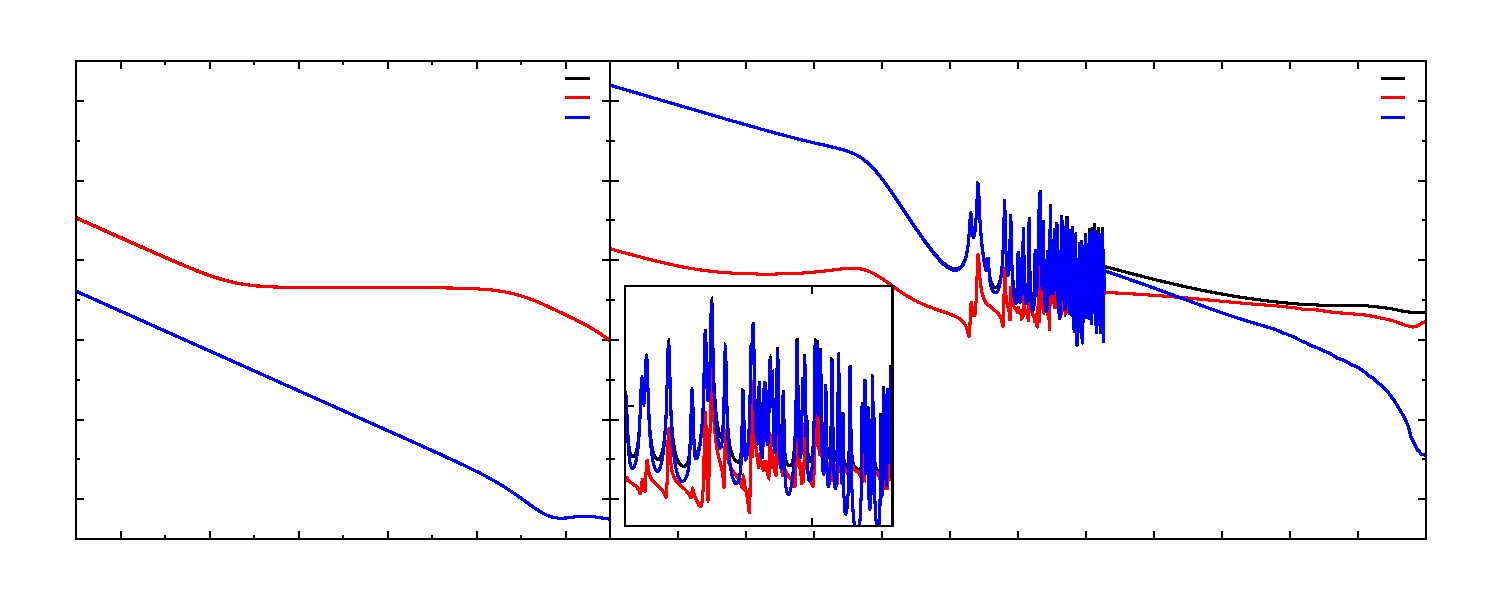
\includegraphics{pics/neutron_xsec}}%
    \gplfronttext
  \end{picture}%
\endgroup
}
	\caption[Neutron cross-sections on hydrogen and gadolinium-157]%
	{Neutron cross-sections on hydrogen (left) and gadolinium (right) as a function of energy from \refref{Brown:2018jhj}. %
	The dominant component for \tapi{1}H is elastic scattering, despite neutron capture %
	reaches relative high cross-section values for subthermal neutrons ($T < 2.5$\,meV).
	Fast neutrons interact on \tapi{157}Gd via elastic scattering, but for lower energies %
	the main contribution comes from neutron capture cross-section.
	The $1/v$ dependency can be appreciated in both cases.
	The inset shows a detail of the resonance region of the cross-section, between 10\,eV and 500\,eV.}
	\label{fig:n_xsec}
\end{figure}


From the considerations above, water turns out to be a good moderator for thermalising fast neutrons.
The energy decrease for water is $\xi_{\text{H}_2\text{O}} \simeq 0.93$, %
when the kinetic energy of the neutron is in the range $2.5\,\text{meV} \lesssim T \lesssim 0.1\,\text{MeV}$.
Neutrons that reach subthermal energies enter the $1/v$ regions in which the capture probabilities increases as $T^{-1}$.
Hydrogen presents a relative high cross-section for neutron capture, as it can be seen from~\reffig{fig:n_xsec}: %
the cross-section for a thermal neutron on hydrogen is measured to be $\np{332.6}$~\,mb~\cite{ZERKIN201831}. %
The cross-section of capture on the oxygen nucleus \tapi{16}O is around $0.19$~\,mb, four orders of magnitude smaller %
than the capture on hydrogen, and therefore typically neglected.
The hydrogen capture is followed by the emission of a $\np{2.2}$\,MeV gamma from the %
de-excitation of the newly-formed deuterium.
The characteristic time for Maxwellian neutrons with energy below 10\,MeV to thermalise and being captured %
by hydrogen in water has been measured to be $(\np{204.8}\pm\np{0.4})$\,\textmu s~\cite{Cokinos:1977zz}.
The typical time and energy of this event require special triggers and dedicated analysis %
to correctly identify the neutron capture on hydrogen in SK.
Since the SK-IV phase, after any primary events above the standard higher energy threshold are detected, 
a time window of 535\,\textmu s is saved with no threshold requirement, so that approximately the 92\,\% %
of neutron capture signals are collected.
The 2.2\,MeV photon produces on average 7$\sim$8 PMT hits, which are difficult to reconstruct accurately.
The PMT hits are expected to happen in a narrow timing distribution and to be anisotropic.
A 10\,ns sliding window is used to look for $\gamma$ candidates with more than 7 hits and less than 50 %
to avoid high energy backgrounds.
With these simple selection criteria, an efficiency of 33.2\,\% is obtained from a simulation of neutron capture events, %
with an expected 4.5 background events per neutrino event.
The background rejection is improved by feeding the simulated data of the selected candidates %
to a neural network, which retains an overall efficiency of 20.5\,\% with \np{0.018} backgrounds per signal event~\cite{Irvine:2014hja}.
The efficiency is found to be highly dependent on the distance travelled by the released neutron, %
due to the fact that knowing the location of the capture significantly reduces the background.

%follows an exponential and the time constant is largely studied amongst all the thermalisation in water.
%It was found that neutron thermalisation in water has a time constant of 5$\mu$s [fujino, sumita, shiba].
%Neutrons can be captured by either the hydrogen or the oxygen.
%Free neutron will capture on a hydrogen nucleus, releasing a 2.2 MeV gamma.
%In SK, for instance, this gamma results in about seven photo-electrons, and thus only detectable with $\simeq$20\,\% %
%efficiency.

\subsection{Neutron calibration}

%https://arxiv.org/pdf/0811.0735.pdf
%https://www.sno.phy.queensu.ca/sno/papers/labranche_phd.pdf
%https://www.sno.phy.queensu.ca/sno/papers/lyon_phd.pdf

Neutron tagging efficiency in SK is measured with an americium-beryllium (Am-Be) source~\cite{Watanabe:2008ru}.
In an Am-Be source, \tapi{214}Am decays 100\,\% of the times into \tapi{237}Np via $\alpha$ emission, %
with a half-life of 432.6\,y.
The $\alpha$ particle is captured by a \tapi{9}Be nucleus to become \tapi{12}C\tapi{*} with the emission of a neutron.
The carbon de-excites to the ground state with sometimes the emission of a 4.43\,MeV photon.
This gamma is used to trigger the neutron emission.
The Am-Be source is placed at the centre of a 5\,cm cube of bismuth germanite (BGO) crystal scintillator and %
the device is lowered inside the water Cherenkov tank.
The gamma ray from the beryllium neutron capture is promptly absorbed by the BGO crystal, %
with the release of scintillation light that triggers the detectors. 
Around a thousands of photoelectrons are typically observed by the PMTs from the BGO emission; %
this intense signal triggers in turn the search for neutron captures on hydrogen.
%Forced triggers were imposed during the SK-III phase to extend the acquisition time window.
The candidates are selected by an analysis similar to the simulation of \refref{Irvine:2014hja}.
Neutrons from beryllium have energies below 10\,MeV, as seen in \reffig{fig:spectra}, %
less than the typical neutron energy resulting from atmospheric neutrino interactions.
For this reason, in the calibration analysis the neutron capture vertex is assumed to be roughly at the same location %
of the Am-Be source.
The efficiency measured in \refref{Watanabe:2008ru} ranges from 13.1\,\% to 24.5\,\%, %
the exact value of which is position dependent.
These values agree overall with the simulation analysis.

\begin{figure}
	\begin{minipage}[t]{0.49\textwidth}
		\centering
		\resizebox{\textwidth}{!}{% GNUPLOT: LaTeX picture with Postscript
\begingroup
  \makeatletter
  \providecommand\color[2][]{%
    \GenericError{(gnuplot) \space\space\space\@spaces}{%
      Package color not loaded in conjunction with
      terminal option `colourtext'%
    }{See the gnuplot documentation for explanation.%
    }{Either use 'blacktext' in gnuplot or load the package
      color.sty in LaTeX.}%
    \renewcommand\color[2][]{}%
  }%
  \providecommand\includegraphics[2][]{%
    \GenericError{(gnuplot) \space\space\space\@spaces}{%
      Package graphicx or graphics not loaded%
    }{See the gnuplot documentation for explanation.%
    }{The gnuplot epslatex terminal needs graphicx.sty or graphics.sty.}%
    \renewcommand\includegraphics[2][]{}%
  }%
  \providecommand\rotatebox[2]{#2}%
  \@ifundefined{ifGPcolor}{%
    \newif\ifGPcolor
    \GPcolortrue
  }{}%
  \@ifundefined{ifGPblacktext}{%
    \newif\ifGPblacktext
    \GPblacktexttrue
  }{}%
  % define a \g@addto@macro without @ in the name:
  \let\gplgaddtomacro\g@addto@macro
  % define empty templates for all commands taking text:
  \gdef\gplbacktext{}%
  \gdef\gplfronttext{}%
  \makeatother
  \ifGPblacktext
    % no textcolor at all
    \def\colorrgb#1{}%
    \def\colorgray#1{}%
  \else
    % gray or color?
    \ifGPcolor
      \def\colorrgb#1{\color[rgb]{#1}}%
      \def\colorgray#1{\color[gray]{#1}}%
      \expandafter\def\csname LTw\endcsname{\color{white}}%
      \expandafter\def\csname LTb\endcsname{\color{black}}%
      \expandafter\def\csname LTa\endcsname{\color{black}}%
      \expandafter\def\csname LT0\endcsname{\color[rgb]{1,0,0}}%
      \expandafter\def\csname LT1\endcsname{\color[rgb]{0,1,0}}%
      \expandafter\def\csname LT2\endcsname{\color[rgb]{0,0,1}}%
      \expandafter\def\csname LT3\endcsname{\color[rgb]{1,0,1}}%
      \expandafter\def\csname LT4\endcsname{\color[rgb]{0,1,1}}%
      \expandafter\def\csname LT5\endcsname{\color[rgb]{1,1,0}}%
      \expandafter\def\csname LT6\endcsname{\color[rgb]{0,0,0}}%
      \expandafter\def\csname LT7\endcsname{\color[rgb]{1,0.3,0}}%
      \expandafter\def\csname LT8\endcsname{\color[rgb]{0.5,0.5,0.5}}%
    \else
      % gray
      \def\colorrgb#1{\color{black}}%
      \def\colorgray#1{\color[gray]{#1}}%
      \expandafter\def\csname LTw\endcsname{\color{white}}%
      \expandafter\def\csname LTb\endcsname{\color{black}}%
      \expandafter\def\csname LTa\endcsname{\color{black}}%
      \expandafter\def\csname LT0\endcsname{\color{black}}%
      \expandafter\def\csname LT1\endcsname{\color{black}}%
      \expandafter\def\csname LT2\endcsname{\color{black}}%
      \expandafter\def\csname LT3\endcsname{\color{black}}%
      \expandafter\def\csname LT4\endcsname{\color{black}}%
      \expandafter\def\csname LT5\endcsname{\color{black}}%
      \expandafter\def\csname LT6\endcsname{\color{black}}%
      \expandafter\def\csname LT7\endcsname{\color{black}}%
      \expandafter\def\csname LT8\endcsname{\color{black}}%
    \fi
  \fi
    \setlength{\unitlength}{0.0500bp}%
    \ifx\gptboxheight\undefined%
      \newlength{\gptboxheight}%
      \newlength{\gptboxwidth}%
      \newsavebox{\gptboxtext}%
    \fi%
    \setlength{\fboxrule}{0.5pt}%
    \setlength{\fboxsep}{1pt}%
\begin{picture}(7200.00,5040.00)%
    \gplgaddtomacro\gplbacktext{%
      \csname LTb\endcsname%%
      \put(747,595){\makebox(0,0)[r]{\strut{}$10^{-4}$}}%
      \csname LTb\endcsname%%
      \put(747,2014){\makebox(0,0)[r]{\strut{}$10^{-3}$}}%
      \csname LTb\endcsname%%
      \put(747,3434){\makebox(0,0)[r]{\strut{}$10^{-2}$}}%
      \csname LTb\endcsname%%
      \put(747,4853){\makebox(0,0)[r]{\strut{}$10^{-1}$}}%
      \csname LTb\endcsname%%
      \put(849,409){\makebox(0,0){\strut{}$0$}}%
      \csname LTb\endcsname%%
      \put(1856,409){\makebox(0,0){\strut{}$2$}}%
      \csname LTb\endcsname%%
      \put(2864,409){\makebox(0,0){\strut{}$4$}}%
      \csname LTb\endcsname%%
      \put(3871,409){\makebox(0,0){\strut{}$6$}}%
      \csname LTb\endcsname%%
      \put(4878,409){\makebox(0,0){\strut{}$8$}}%
      \csname LTb\endcsname%%
      \put(5886,409){\makebox(0,0){\strut{}$10$}}%
      \csname LTb\endcsname%%
      \put(6893,409){\makebox(0,0){\strut{}$12$}}%
    }%
    \gplgaddtomacro\gplfronttext{%
      \csname LTb\endcsname%%
      \put(153,2724){\rotatebox{-270}{\makebox(0,0){\strut{}Distribution}}}%
      \csname LTb\endcsname%%
      \put(3871,130){\makebox(0,0){\strut{}Energy (MeV)}}%
      \csname LTb\endcsname%%
      \put(6411,4081){\makebox(0,0)[r]{\strut{}\tapi{252}Cf $-\ \gamma$}}%
      \csname LTb\endcsname%%
      \put(6411,4360){\makebox(0,0)[r]{\strut{}\tapi{252}Cf $-\ n$}}%
      \csname LTb\endcsname%%
      \put(6411,4639){\makebox(0,0)[r]{\strut{}AmBe $-\ n$}}%
    }%
    \gplbacktext
    \put(0,0){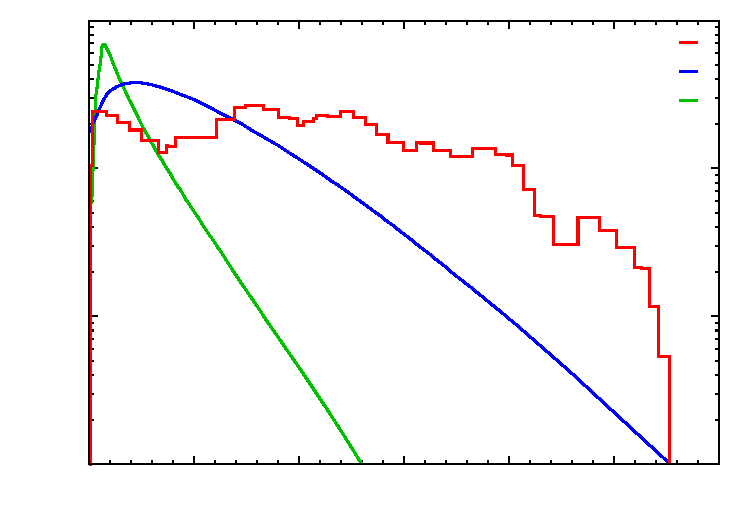
\includegraphics{pics/source_spectrum}}%
    \gplfronttext
  \end{picture}%
\endgroup
}
		\captionof{figure}[Normalised energy distribution of AmBe and \tapi{252}Cf sources]%
		{Normalised energy distribution of neutrons emitted by an AmBe source~\cite{PMID:4744412} %
		and neutrons and photons from the spontaneous fission of a %
		\tapi{252}Cf source~\cite{PhysRev.104.699, PhysRev.108.411}.}
		\label{fig:spectra}
	\end{minipage}
	\hfill
	\begin{minipage}[t]{0.49\textwidth}
		\centering
		\resizebox{\textwidth}{!}{% GNUPLOT: LaTeX picture with Postscript
\begingroup
  \makeatletter
  \providecommand\color[2][]{%
    \GenericError{(gnuplot) \space\space\space\@spaces}{%
      Package color not loaded in conjunction with
      terminal option `colourtext'%
    }{See the gnuplot documentation for explanation.%
    }{Either use 'blacktext' in gnuplot or load the package
      color.sty in LaTeX.}%
    \renewcommand\color[2][]{}%
  }%
  \providecommand\includegraphics[2][]{%
    \GenericError{(gnuplot) \space\space\space\@spaces}{%
      Package graphicx or graphics not loaded%
    }{See the gnuplot documentation for explanation.%
    }{The gnuplot epslatex terminal needs graphicx.sty or graphics.sty.}%
    \renewcommand\includegraphics[2][]{}%
  }%
  \providecommand\rotatebox[2]{#2}%
  \@ifundefined{ifGPcolor}{%
    \newif\ifGPcolor
    \GPcolortrue
  }{}%
  \@ifundefined{ifGPblacktext}{%
    \newif\ifGPblacktext
    \GPblacktexttrue
  }{}%
  % define a \g@addto@macro without @ in the name:
  \let\gplgaddtomacro\g@addto@macro
  % define empty templates for all commands taking text:
  \gdef\gplbacktext{}%
  \gdef\gplfronttext{}%
  \makeatother
  \ifGPblacktext
    % no textcolor at all
    \def\colorrgb#1{}%
    \def\colorgray#1{}%
  \else
    % gray or color?
    \ifGPcolor
      \def\colorrgb#1{\color[rgb]{#1}}%
      \def\colorgray#1{\color[gray]{#1}}%
      \expandafter\def\csname LTw\endcsname{\color{white}}%
      \expandafter\def\csname LTb\endcsname{\color{black}}%
      \expandafter\def\csname LTa\endcsname{\color{black}}%
      \expandafter\def\csname LT0\endcsname{\color[rgb]{1,0,0}}%
      \expandafter\def\csname LT1\endcsname{\color[rgb]{0,1,0}}%
      \expandafter\def\csname LT2\endcsname{\color[rgb]{0,0,1}}%
      \expandafter\def\csname LT3\endcsname{\color[rgb]{1,0,1}}%
      \expandafter\def\csname LT4\endcsname{\color[rgb]{0,1,1}}%
      \expandafter\def\csname LT5\endcsname{\color[rgb]{1,1,0}}%
      \expandafter\def\csname LT6\endcsname{\color[rgb]{0,0,0}}%
      \expandafter\def\csname LT7\endcsname{\color[rgb]{1,0.3,0}}%
      \expandafter\def\csname LT8\endcsname{\color[rgb]{0.5,0.5,0.5}}%
    \else
      % gray
      \def\colorrgb#1{\color{black}}%
      \def\colorgray#1{\color[gray]{#1}}%
      \expandafter\def\csname LTw\endcsname{\color{white}}%
      \expandafter\def\csname LTb\endcsname{\color{black}}%
      \expandafter\def\csname LTa\endcsname{\color{black}}%
      \expandafter\def\csname LT0\endcsname{\color{black}}%
      \expandafter\def\csname LT1\endcsname{\color{black}}%
      \expandafter\def\csname LT2\endcsname{\color{black}}%
      \expandafter\def\csname LT3\endcsname{\color{black}}%
      \expandafter\def\csname LT4\endcsname{\color{black}}%
      \expandafter\def\csname LT5\endcsname{\color{black}}%
      \expandafter\def\csname LT6\endcsname{\color{black}}%
      \expandafter\def\csname LT7\endcsname{\color{black}}%
      \expandafter\def\csname LT8\endcsname{\color{black}}%
    \fi
  \fi
    \setlength{\unitlength}{0.0500bp}%
    \ifx\gptboxheight\undefined%
      \newlength{\gptboxheight}%
      \newlength{\gptboxwidth}%
      \newsavebox{\gptboxtext}%
    \fi%
    \setlength{\fboxrule}{0.5pt}%
    \setlength{\fboxsep}{1pt}%
\begin{picture}(7200.00,5040.00)%
    \gplgaddtomacro\gplbacktext{%
      \csname LTb\endcsname%%
      \put(946,2142){\makebox(0,0)[r]{\strut{}$0.05$}}%
      \put(946,4200){\makebox(0,0)[r]{\strut{}$0.5$}}%
      \put(946,704){\makebox(0,0)[r]{\strut{}$0.01$}}%
      \put(946,2762){\makebox(0,0)[r]{\strut{}$0.1$}}%
      \put(946,4819){\makebox(0,0)[r]{\strut{}$1$}}%
      \put(1460,484){\makebox(0,0){\strut{}$300$}}%
      \put(2223,484){\makebox(0,0){\strut{}$350$}}%
      \put(2986,484){\makebox(0,0){\strut{}$400$}}%
      \put(3750,484){\makebox(0,0){\strut{}$450$}}%
      \put(4513,484){\makebox(0,0){\strut{}$500$}}%
      \put(5276,484){\makebox(0,0){\strut{}$550$}}%
      \put(6040,484){\makebox(0,0){\strut{}$600$}}%
      \put(6803,484){\makebox(0,0){\strut{}$650$}}%
    }%
    \gplgaddtomacro\gplfronttext{%
      \csname LTb\endcsname%%
      \put(198,2761){\rotatebox{-270}{\makebox(0,0){\strut{}Efficiency}}}%
      \put(3940,154){\makebox(0,0){\strut{}Wavelength (nm)}}%
      \csname LTb\endcsname%%
      \put(6212,4624){\makebox(0,0)[r]{\strut{}PMT}}%
      \csname LTb\endcsname%%
      \put(6212,4360){\makebox(0,0)[r]{\strut{}Scintillator}}%
      \csname LTb\endcsname%%
      \put(6212,4096){\makebox(0,0)[r]{\strut{}Correlation}}%
      \csname LTb\endcsname%%
      \put(6212,3832){\makebox(0,0)[r]{\strut{}MC}}%
    }%
    \gplbacktext
    \put(0,0){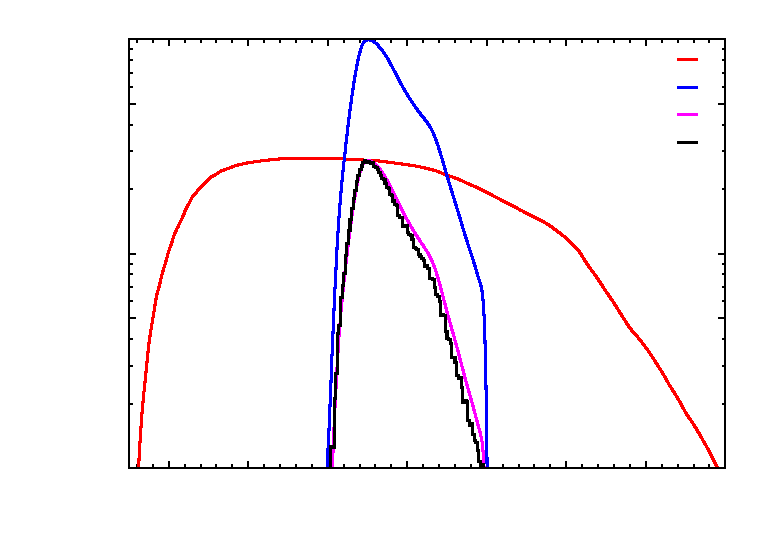
\includegraphics{pics/QE}}%
    \gplfronttext
  \end{picture}%
\endgroup
}
		\captionof{figure}[Distribution of optical photons from the simulation of a neutron calibration device]{%
		Distributions showing PMT quantum efficiency (red), the scintillator yield (blue), %
		their correlation (magenta), and the photons collected by the PMT in the GEANT4 %
		simulation of optical photons (black).}
		\label{fig:QE}
	\end{minipage}
\end{figure}

Another possibility as a source for neutron calibration is using californium-252, which %
undergoes $\alpha$ emissions (96.91\%) or spontaneous fission (SF, 3.09\%).
Thanks to a shorter half-life of 2.645\,y, a \tapi{252}Cf source presents a higher activity compared to an Am-Be source %
with the same number of nucleons.
Furthermore, the SF process emits an average of 3.75 neutrons per fission and an average of 10.3 photons %
summing up to a total energy of 8.2\,Mev~\cite{PhysRev.104.699}.
As for the case of the Am-Be calibrating device, the photons can be collected by a scintillating material %
and tag the emission of neutrons.
After the trigger signal, multiple neutron captures on hydrogen are expected, separated by short intervals in time %
of the order of milliseconds.
The yield of multiple neutrons is an advantage which the SNO collaboration exploited to develop a method, %
called \emph{Time Series Analysis}, that uses multiplicity and time intervals between the detected events %
to find the neutron detection efficiency, the neutron mean life inside the detector, %
and activity from nonfission events~\cite{Labranche:2004sya}.
Differently from the Am-Be source, the activity of which must be known precisely, the neutron tagging calibration %
with a californium source can be done in principle regardless of that information.
The fast-neutron and photon energy spectra from \tapi{252}Cf are shown in \ref{fig:spectra}; %
the neutrons are emitted with a most-probable energy of 0.7\,MeV and an average energy of 2.1\,MeV.
It is reasonable to assume that the capture on hydrogen occurs in the proximity of the source, %
bringing about an even more accurate calibration than with the Am-Be source.


Some preliminary studies were performed to develop a device for neutron calibration %
of a generic water Cherenkov detector.
For laboratory measurements, a \tapi{252}Cf source with an activity of 4.3\,kBq at the time of its production was used.
%measured on the 28\tapi{th} of July, 2017.
The californium is encapsulated in a double-hull stainless steel cylinder, 9.5\,mm in diameter and 37.5\,mm high.
The source is placed in a simple prototype of the device, shown in \reffig{fig:setup}, %
consisting of a cylindrical plastic scintillator (EJ-200), coated with mylar to contain optical photons, %
and optically coupled to an ET Enterprise 9902B series~PMT.
A hole, coaxial to the plastic cylinder, allows to insert the source in the middle of the scintillator.
The cylinder is 3'' in length and 1.5'' in diameter.
The rate of photons emitted by the \tapi{252}Cf source is measured with this setup; %
the signal from the PMT is amplified and cleaned by NIM modules and finally recorded with a 14-bit VME digitiser.
%to count the number of photon triggers from the PMT and %
%a daisy-chain of NIM amplifier, threshold, and discriminator is used before the digitiser to optimise the signal.
Without the source inside the scintillator, a dark rate of 1.633\,Hz is measured, %
whereas with the source the rate increases to 41.395\,Hz.
The distributions of the PMT peaks collected by the digitiser are shown in Fig.~\ref{fig:source}.
A predicted activity of 3.1\,kBq is expected on the day of the measurement---446 days after the production of the source--- %
which translates to a SF rate of 96.46\,Hz.
The SF tagging efficiency with this setup is therefore estimated to be around~41\,\%.

\begin{figure}
	\begin{minipage}[t]{0.53\textwidth}
		\centering
		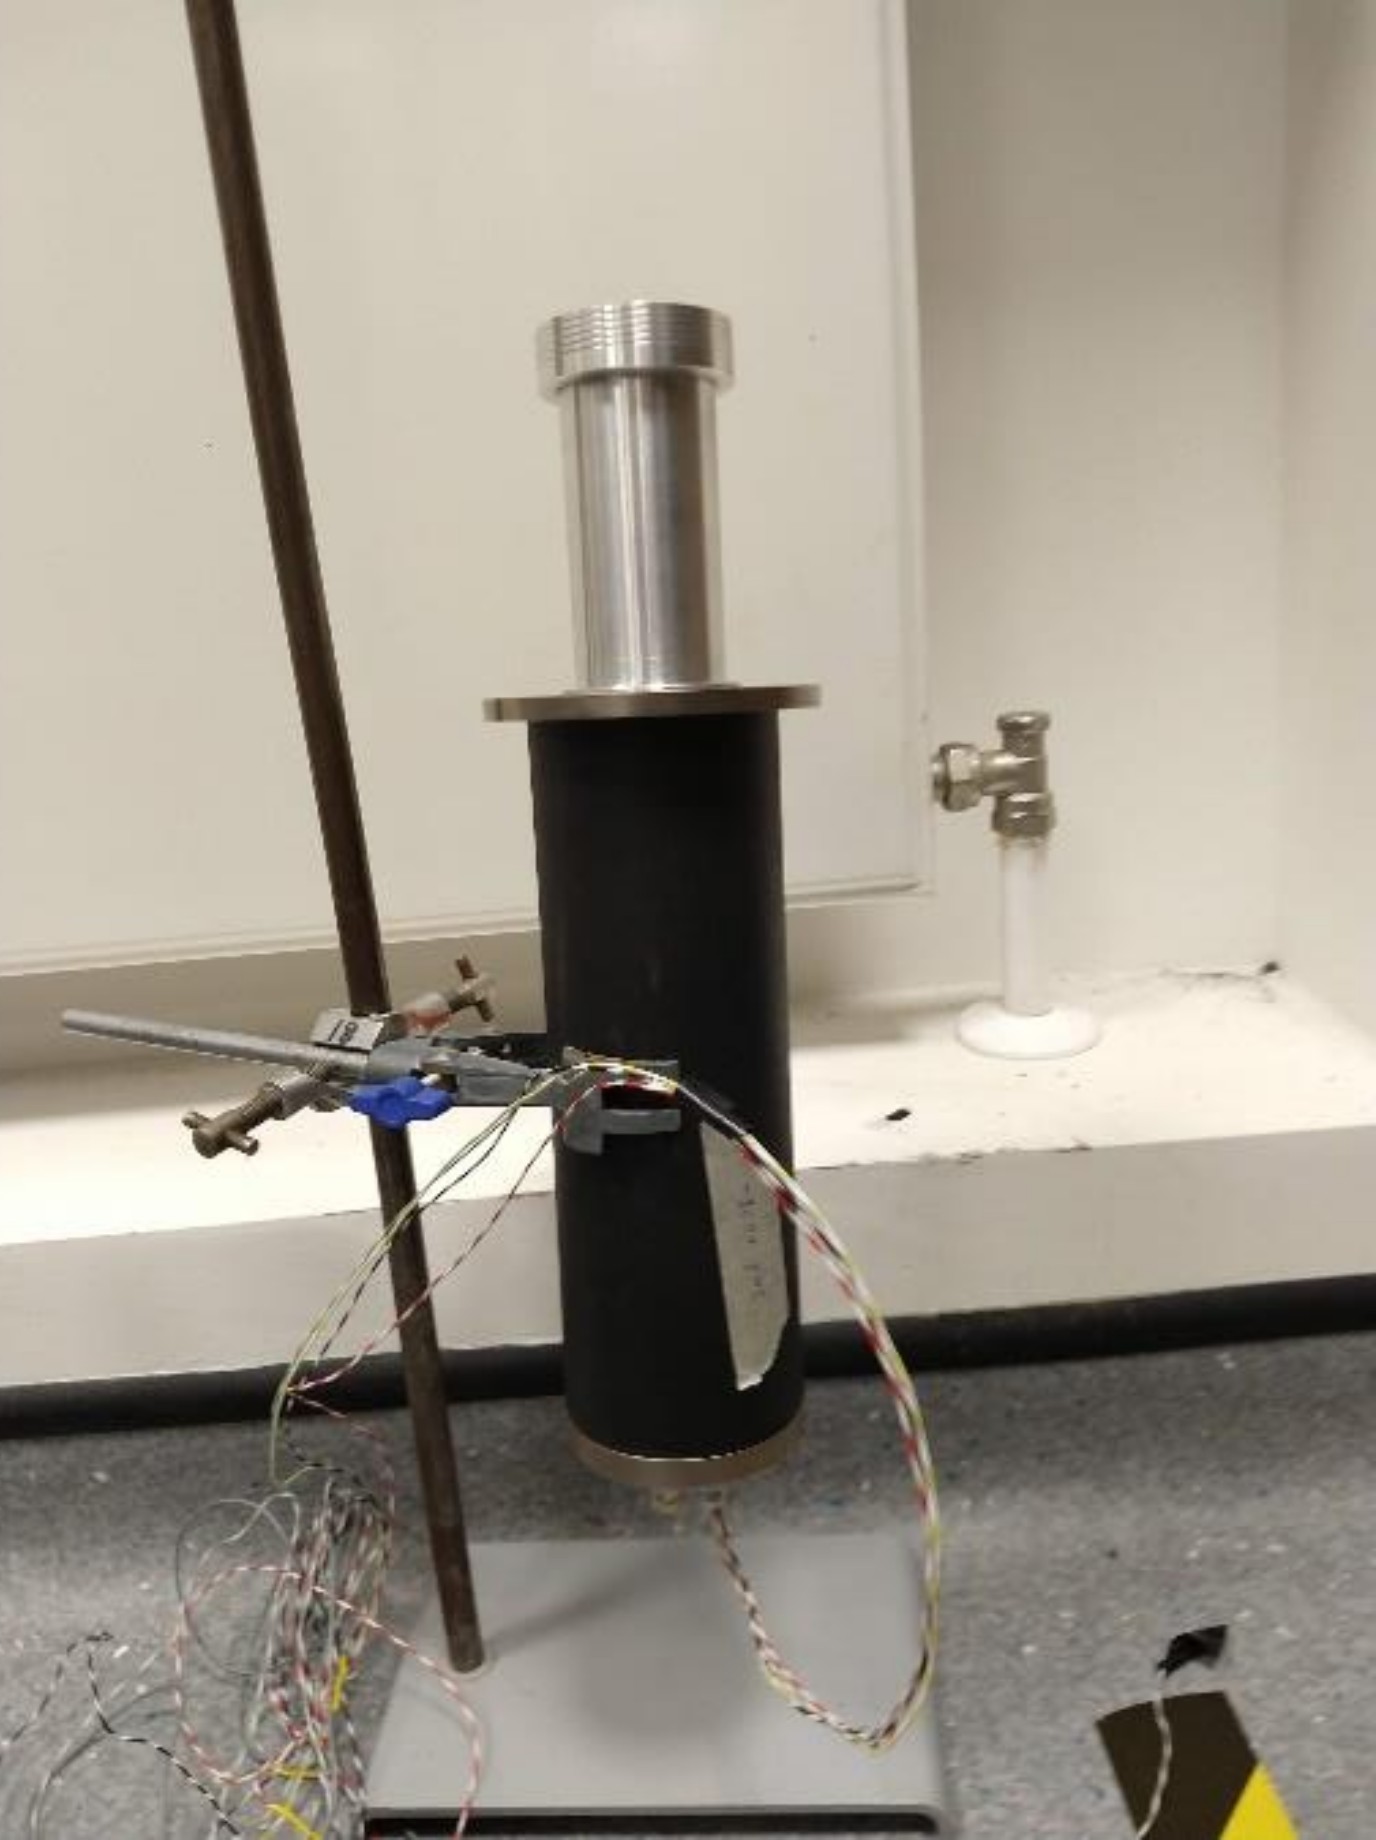
\includegraphics[width=0.48\linewidth]{pics/device.png}
		\raisebox{2.8em}{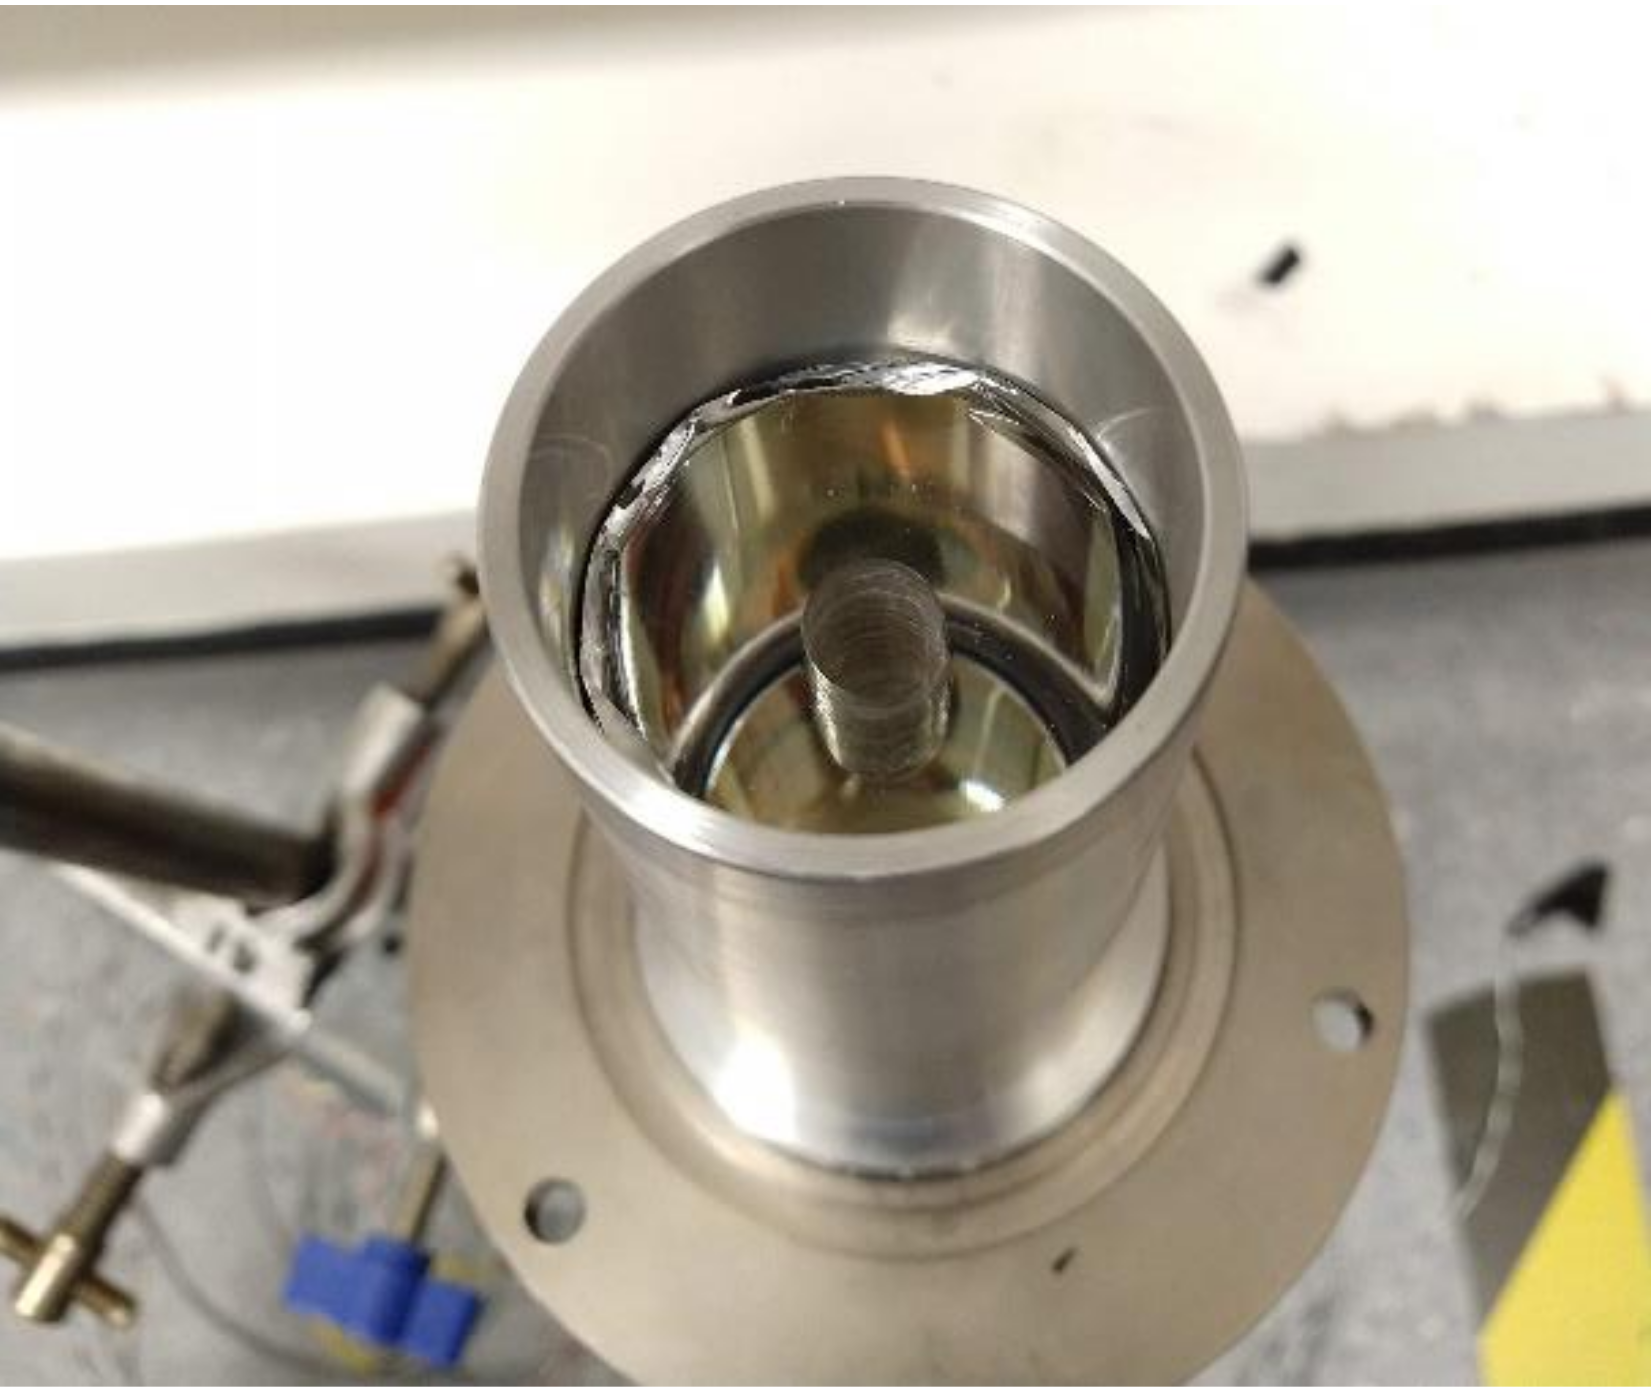
\includegraphics[width=0.48\linewidth]{pics/device_in.png}}
		\captionof{figure}[Setup used to test a californium source]%
		{Setup used to test the californium source.
		The plastic scintillator cylinder is encased in an aluminium structure %
		connected to the PMT support (black).
		The scintillator is optically coupled to the PMT.}
		\label{fig:setup}
	\end{minipage}
	\hfill
	\begin{minipage}[t]{0.45\textwidth}
		\centering
		\resizebox{\textwidth}{!}{% GNUPLOT: LaTeX picture with Postscript
\begingroup
  \makeatletter
  \providecommand\color[2][]{%
    \GenericError{(gnuplot) \space\space\space\@spaces}{%
      Package color not loaded in conjunction with
      terminal option `colourtext'%
    }{See the gnuplot documentation for explanation.%
    }{Either use 'blacktext' in gnuplot or load the package
      color.sty in LaTeX.}%
    \renewcommand\color[2][]{}%
  }%
  \providecommand\includegraphics[2][]{%
    \GenericError{(gnuplot) \space\space\space\@spaces}{%
      Package graphicx or graphics not loaded%
    }{See the gnuplot documentation for explanation.%
    }{The gnuplot epslatex terminal needs graphicx.sty or graphics.sty.}%
    \renewcommand\includegraphics[2][]{}%
  }%
  \providecommand\rotatebox[2]{#2}%
  \@ifundefined{ifGPcolor}{%
    \newif\ifGPcolor
    \GPcolortrue
  }{}%
  \@ifundefined{ifGPblacktext}{%
    \newif\ifGPblacktext
    \GPblacktexttrue
  }{}%
  % define a \g@addto@macro without @ in the name:
  \let\gplgaddtomacro\g@addto@macro
  % define empty templates for all commands taking text:
  \gdef\gplbacktext{}%
  \gdef\gplfronttext{}%
  \makeatother
  \ifGPblacktext
    % no textcolor at all
    \def\colorrgb#1{}%
    \def\colorgray#1{}%
  \else
    % gray or color?
    \ifGPcolor
      \def\colorrgb#1{\color[rgb]{#1}}%
      \def\colorgray#1{\color[gray]{#1}}%
      \expandafter\def\csname LTw\endcsname{\color{white}}%
      \expandafter\def\csname LTb\endcsname{\color{black}}%
      \expandafter\def\csname LTa\endcsname{\color{black}}%
      \expandafter\def\csname LT0\endcsname{\color[rgb]{1,0,0}}%
      \expandafter\def\csname LT1\endcsname{\color[rgb]{0,1,0}}%
      \expandafter\def\csname LT2\endcsname{\color[rgb]{0,0,1}}%
      \expandafter\def\csname LT3\endcsname{\color[rgb]{1,0,1}}%
      \expandafter\def\csname LT4\endcsname{\color[rgb]{0,1,1}}%
      \expandafter\def\csname LT5\endcsname{\color[rgb]{1,1,0}}%
      \expandafter\def\csname LT6\endcsname{\color[rgb]{0,0,0}}%
      \expandafter\def\csname LT7\endcsname{\color[rgb]{1,0.3,0}}%
      \expandafter\def\csname LT8\endcsname{\color[rgb]{0.5,0.5,0.5}}%
    \else
      % gray
      \def\colorrgb#1{\color{black}}%
      \def\colorgray#1{\color[gray]{#1}}%
      \expandafter\def\csname LTw\endcsname{\color{white}}%
      \expandafter\def\csname LTb\endcsname{\color{black}}%
      \expandafter\def\csname LTa\endcsname{\color{black}}%
      \expandafter\def\csname LT0\endcsname{\color{black}}%
      \expandafter\def\csname LT1\endcsname{\color{black}}%
      \expandafter\def\csname LT2\endcsname{\color{black}}%
      \expandafter\def\csname LT3\endcsname{\color{black}}%
      \expandafter\def\csname LT4\endcsname{\color{black}}%
      \expandafter\def\csname LT5\endcsname{\color{black}}%
      \expandafter\def\csname LT6\endcsname{\color{black}}%
      \expandafter\def\csname LT7\endcsname{\color{black}}%
      \expandafter\def\csname LT8\endcsname{\color{black}}%
    \fi
  \fi
    \setlength{\unitlength}{0.0500bp}%
    \ifx\gptboxheight\undefined%
      \newlength{\gptboxheight}%
      \newlength{\gptboxwidth}%
      \newsavebox{\gptboxtext}%
    \fi%
    \setlength{\fboxrule}{0.5pt}%
    \setlength{\fboxsep}{1pt}%
\begin{picture}(7200.00,5040.00)%
    \gplgaddtomacro\gplbacktext{%
      \csname LTb\endcsname%%
      \put(1078,704){\makebox(0,0)[r]{\strut{}$10^{-3}$}}%
      \put(1078,1733){\makebox(0,0)[r]{\strut{}$10^{-2}$}}%
      \put(1078,2762){\makebox(0,0)[r]{\strut{}$0.1$}}%
      \put(1078,3790){\makebox(0,0)[r]{\strut{}$1$}}%
      \put(1078,4819){\makebox(0,0)[r]{\strut{}$10$}}%
      \put(1210,484){\makebox(0,0){\strut{}$0$}}%
      \put(2142,484){\makebox(0,0){\strut{}$0.1$}}%
      \put(3074,484){\makebox(0,0){\strut{}$0.2$}}%
      \put(4007,484){\makebox(0,0){\strut{}$0.3$}}%
      \put(4939,484){\makebox(0,0){\strut{}$0.4$}}%
      \put(5871,484){\makebox(0,0){\strut{}$0.5$}}%
      \put(6803,484){\makebox(0,0){\strut{}$0.6$}}%
    }%
    \gplgaddtomacro\gplfronttext{%
      \csname LTb\endcsname%%
      \put(298,2761){\rotatebox{-270}{\makebox(0,0){\strut{}Events / s}}}%
      \put(4006,154){\makebox(0,0){\strut{}Peak (V)}}%
      \csname LTb\endcsname%%
      \put(6212,4624){\makebox(0,0)[r]{\strut{}Source in}}%
      \csname LTb\endcsname%%
      \put(6212,4360){\makebox(0,0)[r]{\strut{}Source out}}%
    }%
    \gplbacktext
    \put(0,0){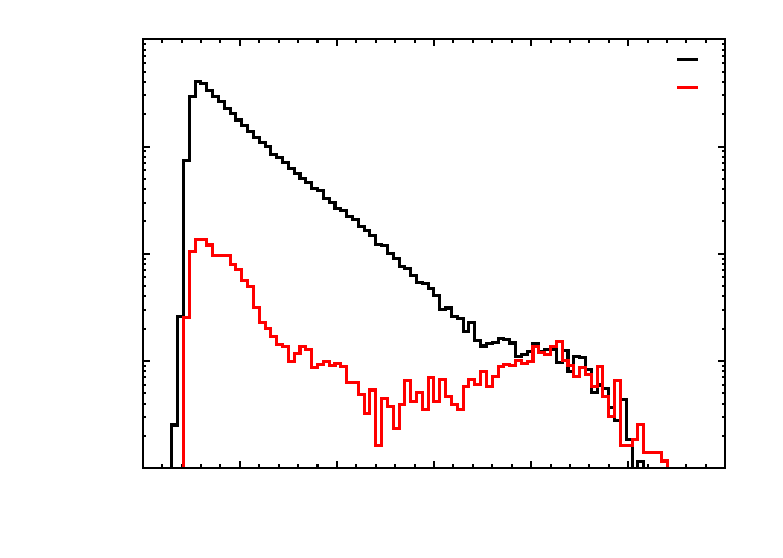
\includegraphics{pics/peaksources}}%
    \gplfronttext
  \end{picture}%
\endgroup
}
		\captionof{figure}[Distribution of PMT peaks measured with a californium source]%
		{Distribution of PMT peaks measured with source inside (black) and source removed from the scintillator~(red).}
		\label{fig:source}
	\end{minipage}
\end{figure}

A GEANT4~\cite{Agostinelli:2002hh} simulation of the setup was performed with the aim of optimising the calibration instrument.
An ideal device would absorb all the photons converting them into visible light without affecting the neutrons.
The plot in \reffig{fig:QE} shows the correct implementation of the scintillator and PMT efficiencies in the simulation: %
there is good agreement with the MC distribution and the expected optical photon spectrum.
Different volumes and materials are tested for the scintillator in the simulation.
As far as materials are concerned, BGO crystal and a generic vinyltouluene are chosen.
The selected shapes for the volume are a cube and cylinders with a diameter-height-ratio 1:1 and 1:2.
The latter shape models the prototype tested in the laboratory.
The characteristic size, i.e.\ the side for the cube and the height for the cylinders, is varied from 1\,cm to 40\,cm.
The simulation tracks the energy deposited in the scintillator by the photons and the number of neutrons escaping the device, %
from a simulation of \np{10000} SF events.
The result is shown in Fig.~\ref{fig:geant4}, where for both photons and neutrons %
the average value of the fraction of absorbed energy with respect to the initial one is plotted against the size.
In terms of materials, the BGO crystal unsurprisingly performs better than the plastic scintillator, %
absorbing almost the entirety of photons and leaving the neutrons mainly unaffected.
Apart from not being as efficient as scintillator, the hydrogen in the plastic thermalises the neutrons more than BGO.
This would impact the capture time in a water Cherenkov detector.
In terms of sizes and shapes, a BGO cube of $4\sim6$\,cm sides seems to maximise photon absorption and minimise %
the energy loss of neutrons.
This is in line with the choice for the calibrating device for SK, which is a 5\,cm BGO cube.
Both the cylindrical shapes are optimal when the height is $7\sim11$\,cm, but more crystal would be required %
increasing the cost of the device.
As far as the plastic scintillator is concerned, it is more difficult to define an optimal size/shape figure:
a cubic scintillator is more efficient in collecting photons, but being the form with the largest volume %
per given size, it is also more effective in slowing down neutrons.
The two cylinder shapes have similar performances, proportionally to their volumes.
Further R\&D is in place to build an optimal device for neutron calibration.

\begin{figure}
	\centering
	\resizebox{\textwidth}{!}{% GNUPLOT: LaTeX picture with Postscript
\begingroup
  \makeatletter
  \providecommand\color[2][]{%
    \GenericError{(gnuplot) \space\space\space\@spaces}{%
      Package color not loaded in conjunction with
      terminal option `colourtext'%
    }{See the gnuplot documentation for explanation.%
    }{Either use 'blacktext' in gnuplot or load the package
      color.sty in LaTeX.}%
    \renewcommand\color[2][]{}%
  }%
  \providecommand\includegraphics[2][]{%
    \GenericError{(gnuplot) \space\space\space\@spaces}{%
      Package graphicx or graphics not loaded%
    }{See the gnuplot documentation for explanation.%
    }{The gnuplot epslatex terminal needs graphicx.sty or graphics.sty.}%
    \renewcommand\includegraphics[2][]{}%
  }%
  \providecommand\rotatebox[2]{#2}%
  \@ifundefined{ifGPcolor}{%
    \newif\ifGPcolor
    \GPcolortrue
  }{}%
  \@ifundefined{ifGPblacktext}{%
    \newif\ifGPblacktext
    \GPblacktexttrue
  }{}%
  % define a \g@addto@macro without @ in the name:
  \let\gplgaddtomacro\g@addto@macro
  % define empty templates for all commands taking text:
  \gdef\gplbacktext{}%
  \gdef\gplfronttext{}%
  \makeatother
  \ifGPblacktext
    % no textcolor at all
    \def\colorrgb#1{}%
    \def\colorgray#1{}%
  \else
    % gray or color?
    \ifGPcolor
      \def\colorrgb#1{\color[rgb]{#1}}%
      \def\colorgray#1{\color[gray]{#1}}%
      \expandafter\def\csname LTw\endcsname{\color{white}}%
      \expandafter\def\csname LTb\endcsname{\color{black}}%
      \expandafter\def\csname LTa\endcsname{\color{black}}%
      \expandafter\def\csname LT0\endcsname{\color[rgb]{1,0,0}}%
      \expandafter\def\csname LT1\endcsname{\color[rgb]{0,1,0}}%
      \expandafter\def\csname LT2\endcsname{\color[rgb]{0,0,1}}%
      \expandafter\def\csname LT3\endcsname{\color[rgb]{1,0,1}}%
      \expandafter\def\csname LT4\endcsname{\color[rgb]{0,1,1}}%
      \expandafter\def\csname LT5\endcsname{\color[rgb]{1,1,0}}%
      \expandafter\def\csname LT6\endcsname{\color[rgb]{0,0,0}}%
      \expandafter\def\csname LT7\endcsname{\color[rgb]{1,0.3,0}}%
      \expandafter\def\csname LT8\endcsname{\color[rgb]{0.5,0.5,0.5}}%
    \else
      % gray
      \def\colorrgb#1{\color{black}}%
      \def\colorgray#1{\color[gray]{#1}}%
      \expandafter\def\csname LTw\endcsname{\color{white}}%
      \expandafter\def\csname LTb\endcsname{\color{black}}%
      \expandafter\def\csname LTa\endcsname{\color{black}}%
      \expandafter\def\csname LT0\endcsname{\color{black}}%
      \expandafter\def\csname LT1\endcsname{\color{black}}%
      \expandafter\def\csname LT2\endcsname{\color{black}}%
      \expandafter\def\csname LT3\endcsname{\color{black}}%
      \expandafter\def\csname LT4\endcsname{\color{black}}%
      \expandafter\def\csname LT5\endcsname{\color{black}}%
      \expandafter\def\csname LT6\endcsname{\color{black}}%
      \expandafter\def\csname LT7\endcsname{\color{black}}%
      \expandafter\def\csname LT8\endcsname{\color{black}}%
    \fi
  \fi
    \setlength{\unitlength}{0.0500bp}%
    \ifx\gptboxheight\undefined%
      \newlength{\gptboxheight}%
      \newlength{\gptboxwidth}%
      \newsavebox{\gptboxtext}%
    \fi%
    \setlength{\fboxrule}{0.5pt}%
    \setlength{\fboxsep}{1pt}%
\begin{picture}(14400.00,7200.00)%
    \gplgaddtomacro\gplbacktext{%
      \csname LTb\endcsname%%
      \put(618,540){\makebox(0,0)[r]{\strut{}0}}%
      \csname LTb\endcsname%%
      \put(618,1726){\makebox(0,0)[r]{\strut{}0.2}}%
      \csname LTb\endcsname%%
      \put(618,2912){\makebox(0,0)[r]{\strut{}0.4}}%
      \csname LTb\endcsname%%
      \put(618,4098){\makebox(0,0)[r]{\strut{}0.6}}%
      \csname LTb\endcsname%%
      \put(618,5284){\makebox(0,0)[r]{\strut{}0.8}}%
      \csname LTb\endcsname%%
      \put(618,6470){\makebox(0,0)[r]{\strut{}1}}%
      \csname LTb\endcsname%%
      \put(720,354){\makebox(0,0){\strut{}$0$}}%
      \csname LTb\endcsname%%
      \put(1570,354){\makebox(0,0){\strut{}$5$}}%
      \csname LTb\endcsname%%
      \put(2421,354){\makebox(0,0){\strut{}$10$}}%
      \csname LTb\endcsname%%
      \put(3271,354){\makebox(0,0){\strut{}$15$}}%
      \csname LTb\endcsname%%
      \put(4122,354){\makebox(0,0){\strut{}$20$}}%
      \csname LTb\endcsname%%
      \put(4972,354){\makebox(0,0){\strut{}$25$}}%
      \csname LTb\endcsname%%
      \put(5822,354){\makebox(0,0){\strut{}$30$}}%
      \csname LTb\endcsname%%
      \put(6673,354){\makebox(0,0){\strut{}$35$}}%
    }%
    \gplgaddtomacro\gplfronttext{%
      \csname LTb\endcsname%%
      \put(126,3653){\rotatebox{-270}{\makebox(0,0){\strut{}Average fraction of absorbed energy (\%)}}}%
      \csname LTb\endcsname%%
      \put(4121,75){\makebox(0,0){\strut{}Size (cm)}}%
      \csname LTb\endcsname%%
      \put(4121,7046){\makebox(0,0){\strut{}BGO scintillator}}%
      \csname LTb\endcsname%%
      \put(6990,1451){\makebox(0,0)[r]{\strut{}Cube}}%
      \csname LTb\endcsname%%
      \put(6990,1265){\makebox(0,0)[r]{\strut{}Cyl.\ 1:1}}%
      \csname LTb\endcsname%%
      \put(6990,1079){\makebox(0,0)[r]{\strut{}Cyl.\ 1:2}}%
      \csname LTb\endcsname%%
      \put(6990,893){\makebox(0,0)[r]{\strut{}$\gamma$}}%
      \csname LTb\endcsname%%
      \put(6990,707){\makebox(0,0)[r]{\strut{}$n$}}%
    }%
    \gplgaddtomacro\gplbacktext{%
      \csname LTb\endcsname%%
      \put(7421,540){\makebox(0,0)[r]{\strut{}}}%
      \csname LTb\endcsname%%
      \put(7421,1726){\makebox(0,0)[r]{\strut{}}}%
      \csname LTb\endcsname%%
      \put(7421,2912){\makebox(0,0)[r]{\strut{}}}%
      \csname LTb\endcsname%%
      \put(7421,4098){\makebox(0,0)[r]{\strut{}}}%
      \csname LTb\endcsname%%
      \put(7421,5284){\makebox(0,0)[r]{\strut{}}}%
      \csname LTb\endcsname%%
      \put(7421,6470){\makebox(0,0)[r]{\strut{}}}%
      \csname LTb\endcsname%%
      \put(7523,354){\makebox(0,0){\strut{}$0$}}%
      \csname LTb\endcsname%%
      \put(8374,354){\makebox(0,0){\strut{}$5$}}%
      \csname LTb\endcsname%%
      \put(9224,354){\makebox(0,0){\strut{}$10$}}%
      \csname LTb\endcsname%%
      \put(10075,354){\makebox(0,0){\strut{}$15$}}%
      \csname LTb\endcsname%%
      \put(10925,354){\makebox(0,0){\strut{}$20$}}%
      \csname LTb\endcsname%%
      \put(11776,354){\makebox(0,0){\strut{}$25$}}%
      \csname LTb\endcsname%%
      \put(12626,354){\makebox(0,0){\strut{}$30$}}%
      \csname LTb\endcsname%%
      \put(13477,354){\makebox(0,0){\strut{}$35$}}%
      \csname LTb\endcsname%%
      \put(14327,354){\makebox(0,0){\strut{}$40$}}%
    }%
    \gplgaddtomacro\gplfronttext{%
      \csname LTb\endcsname%%
      \put(10925,75){\makebox(0,0){\strut{}Size (cm)}}%
      \csname LTb\endcsname%%
      \put(10925,7046){\makebox(0,0){\strut{}Plastic scintillator}}%
      \csname LTb\endcsname%%
      \put(13794,1451){\makebox(0,0)[r]{\strut{}Cube}}%
      \csname LTb\endcsname%%
      \put(13794,1265){\makebox(0,0)[r]{\strut{}Cyl.\ 1:1}}%
      \csname LTb\endcsname%%
      \put(13794,1079){\makebox(0,0)[r]{\strut{}Cyl.\ 1:2}}%
      \csname LTb\endcsname%%
      \put(13794,893){\makebox(0,0)[r]{\strut{}$\gamma$}}%
      \csname LTb\endcsname%%
      \put(13794,707){\makebox(0,0)[r]{\strut{}$n$}}%
    }%
    \gplbacktext
    \put(0,0){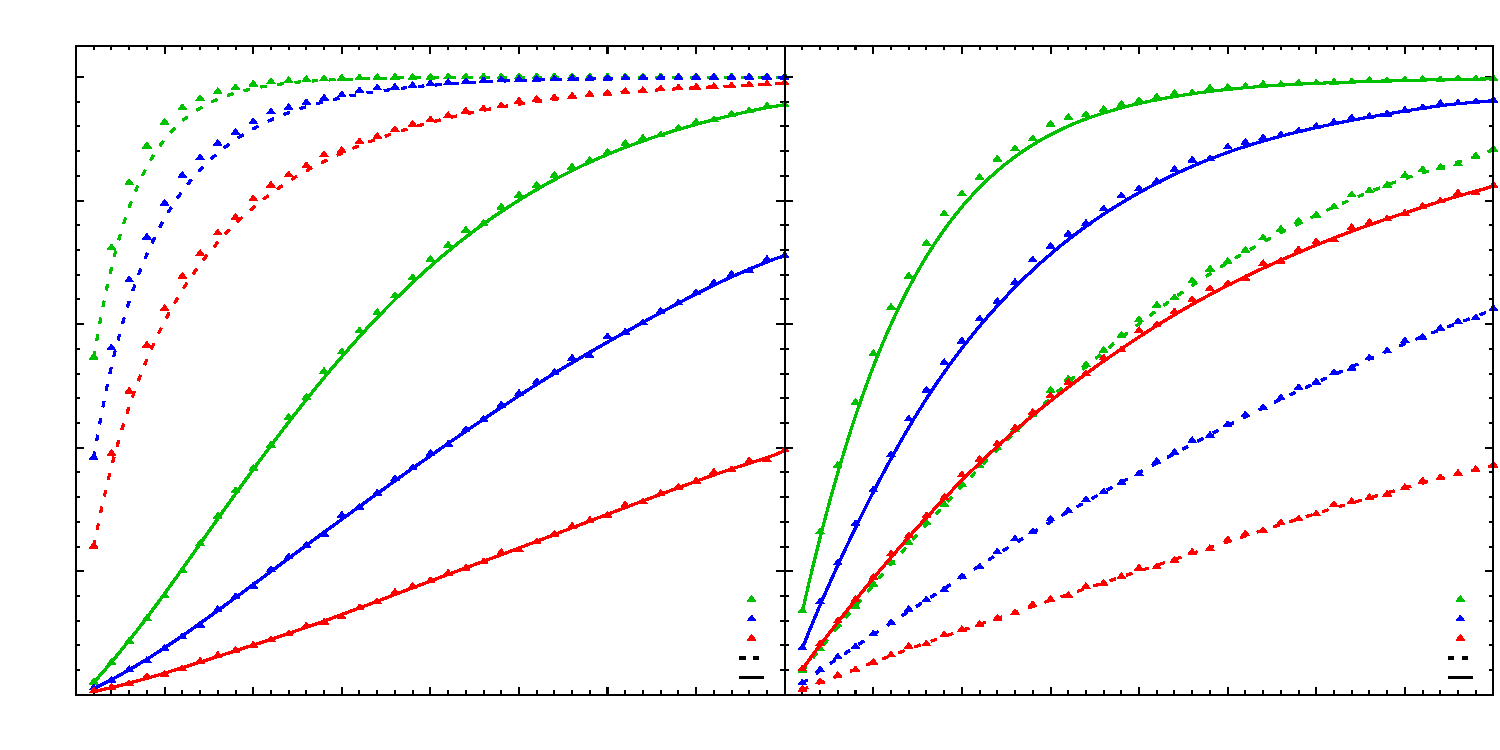
\includegraphics{n_vs_gamma_2}}%
    \gplfronttext
  \end{picture}%
\endgroup
}
	\caption[Performance of different scintillators from the simulation of a neutron calibration device]%
	{Result of the GEANT4 simulation (points), showing the performance of different scintillators.
	The lines are a smooth interpolation between simulation points.
	The fraction of absorbed energy per initial energy of neutrons (solid) and photons (dashed) %
	is averaged and plotted against the scintillator size.
	Three shapes are tested: a cube (green), a cylinder with diameter-height-ratio of 1:1 (blue), %
	and a cylinder with ratio 1:2 (red).
	On the left, the scintillating material is BGO crystal; on the right, %
	a generic vinyltouluene plastic is used.}
	\label{fig:geant4}
\end{figure}


%To verify neutron tagging efficiency given above, experimental tests were conducted with an Am/Be source embedded in a bismuth germanite (BGO) scintillator. The prompt and delayed event-pair is generated via: α + 9Be →12
%C∗+n; 12C∗ →12 C+γ(prompt); n+p → d+γ(delayed).
%The scintillation light induced by 4.43 MeV deexcitation γ
%serves as the primary event. Note that the reaction to the
%ground state of 12C also exists, where no 4.43 MeV deexcitation γ is emitted. The experimental apparatus was
%deployed at the center of the tank, during which the trigger
%gate to catch 2.2 MeV γ was temporarily enlarged to 800
%μs in order to obtain a complete neutron capture time spectrum. To estimate source related background (e.g. ground
%transition neutron), 10 Hz 800μs random trigger data was
%also taken.
%The final N10 distribution after all cuts applied is shown in
%Fig. 2, where for Am/Be data all backgrounds are subtracted according to random trigger data. Signal efficiencies for
%MC and data are (19.2±0.1)% and (19.0±0.2)%, respectively. Data is in good agreement with MC. Fig. 3 shows
%the distribution of time difference (ΔT) between delayed
%neutron signal and prompt event. The neutron lifetime in
%pure water is measured to be (201.8 ± 4.7)μs using a unbinned maximum likelihood fitting as shown in Fig. 3.
%
%The Am-Be source is embedded in a 5 cm cube of BGO scintillator (see figure 8.27)
%to amplify the light released by the 4.4 MeV γ-ray, such that it will activate the SHE
%trigger in the detector. Upon triggering SHE stores 35µs of data, and then an extended
%AFT trigger is activated to store an additional 800µs, and grant a more complete view
%the neutron capture time spectrum.
%Figure 8.27: Am-Be crystal embedded in a 5 cm cube of BGO scintillator. This is
%held in an acrylic case.
%This configuration was set up in 3 different locations around the tank: the centre (35.3,
%-70.7, 0) cm (Centre), near the side of the barrel (35.3, -1201.9, 0) cm (Y12), and near
%the top of the tank (35.3, -70.7, 1500.0) cm (Z15). Random data was also taken with
%the apparatus in the centre, using a 10Hz trigger, to study the irreducible background
%from the ground-state transition.
%
%
%Neutron tagging is then performed on the remaining Am-Be dataset, and a 2.2 MeV
%γ-ray MC. There are some differences between this study and the atmospheric neutrino study discussed up until now. Neutrons released by Beryllium have an energy
%ranging from 2-10 MeV, much less than the average neutron energy following atmospheric neutrino interactions. Thus, we can make the assumption that the location of
%the Am-Be apparatus is roughly the same as the neutron capture vertex. This raises
%the expected neutron detection efficiency in accordance with figure 8.23. In addition,
%Chapter 8. Neutron Tagging 140
%the PMT after-pulse observed following high energy atmospheric neutrino events (figure 8.5) is not produced to the same extent after Am-Be events, so neutron searching
%is started at 5µs (previously > 18µs) after the primary trigger. The AFT trigger for
%Am-Be is also extended, allowing neutron-searching until 835µs after the initial trigger.
%The efficiency is calculated by fitting the timing distribution of neutron candidates to a
%constant background + exponentially decaying signal representing the neutron capture
%lifetime.

